\centerline{\bf \Huge Точка Микеля}

\textbf{Теорема.}
\textit{Четыре прямые общего положения (то есть среди них нет параллельных, и никакие три из них не пересекаются в одной точке) высекают на плоскости четыре треугольника. Описанные окружности этих треугольников пересекаются в одной точке. Эту точку называют точкой Микеля.}

\begin{figure}[h]
    \centering
    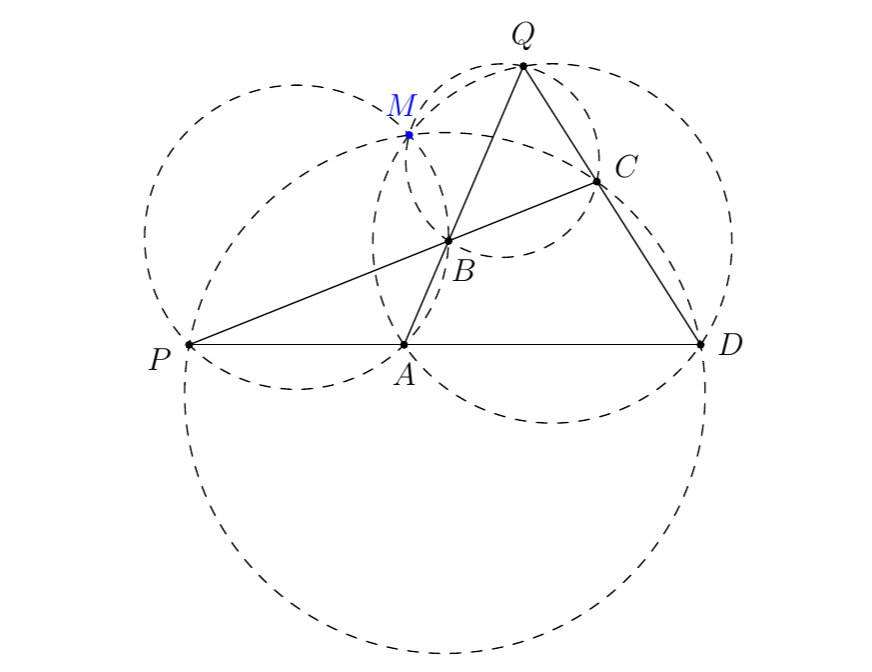
\includegraphics[width=0.8\linewidth]{ЭлМШ 2025-2026/I блок/10/VII/mpt_1.png}
    \caption{}
    \label{fig:placeholder}
\end{figure}

\textit{Доказательство.}
Введём обозначения, как на рис. 1.
Пусть описанные окружности треугольников $P A B$ и $Q C B$ пересекаются в точке $M$. Покажем, что описанная окружность треугольника $P C D$ проходит через $M$. $\angle B M C=\angle B Q C$, так как они опираются на одну дугу. Так как четырёхугольник $M P A B$ вписанный, $\angle P M B=\angle B A D$. Так как сумма углов треугольника равна $180^{\circ}$,

$$
180^{\circ}-\angle A D Q=\angle B A D+\angle B Q C=\angle P M B+\angle B M C=\angle P M C
$$


Значит, четырёхугольник $P M C D$ - вписанный.
Аналогично, $M$ лежит на описанной окружности треугольника $Q A D$.


\newpage

\hspace{3mm}

\textbf{\Large Направленные углы}

Проблема приведённого <<доказательства>> в том, что оно сильно опирается на картинку. Чтобы не разбирать много случаев, можно записать решение с помощью направленных углов.

\textbf{Дисклеймер}: в терминах направленных углов тяжело придумать решение, но решение, работающее в частном случае, бывает легко перевести на их язык.

\textbf{Определение 1}. $\ell_1$ и $\ell_2$ - две прямые на плоскости. Направленным углом $\angle\left(\ell_1, \ell_2\right)$ называют угол такой, что поворот на него против часовой стрелки переведёт $\ell_1$ в прямую, параллельную $\ell_2$.

\begin{figure}[h]
    \centering
    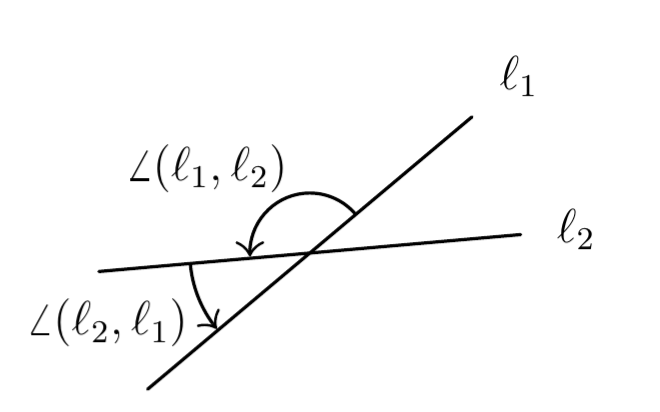
\includegraphics[width=0.35\linewidth]{ЭлМШ 2025-2026/I блок/10/VII/mpt_2.png}
    \caption{}
    \label{fig:placeholder}
\end{figure}

\textbf{Теорема.} \textit{Четыре точки $A, B, C, D$ лежат на одной окружности тогда и только тогда, когда $\angle(A B, A C)=\angle(D B, D C)$}

\begin{figure}[h]
    \centering
    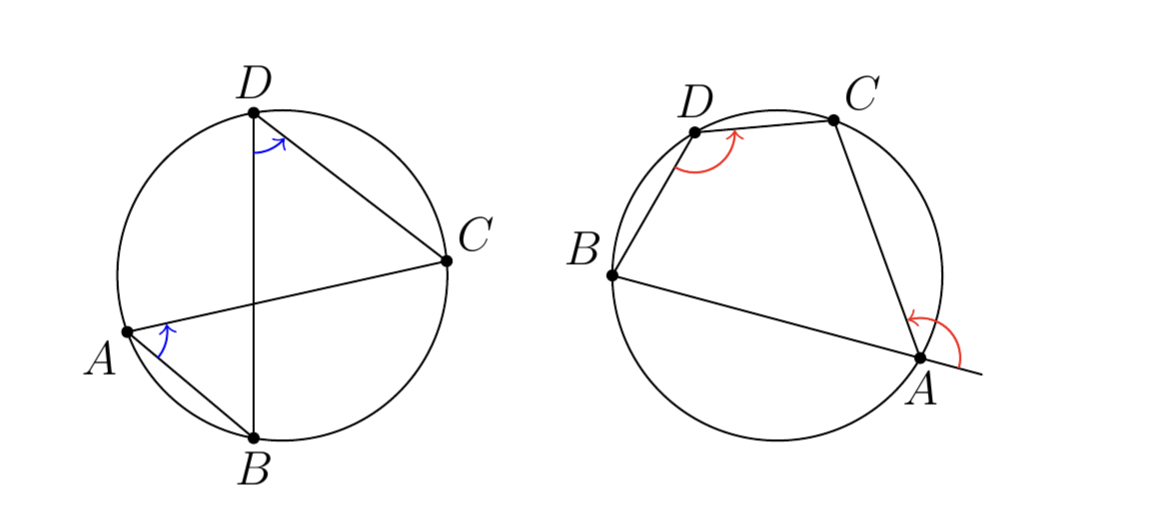
\includegraphics[width=0.8\linewidth]{ЭлМШ 2025-2026/I блок/10/VII/mpt_3.png}
    \caption{}
    \label{fig:placeholder}
\end{figure}

\newpage

\hspace{3mm}

\textbf{\Large Новое решение через направленные углы}

Покажем, как перевести решение на язык направленных углов на примере доказательства существования точки Микеля.

\begin{center}
    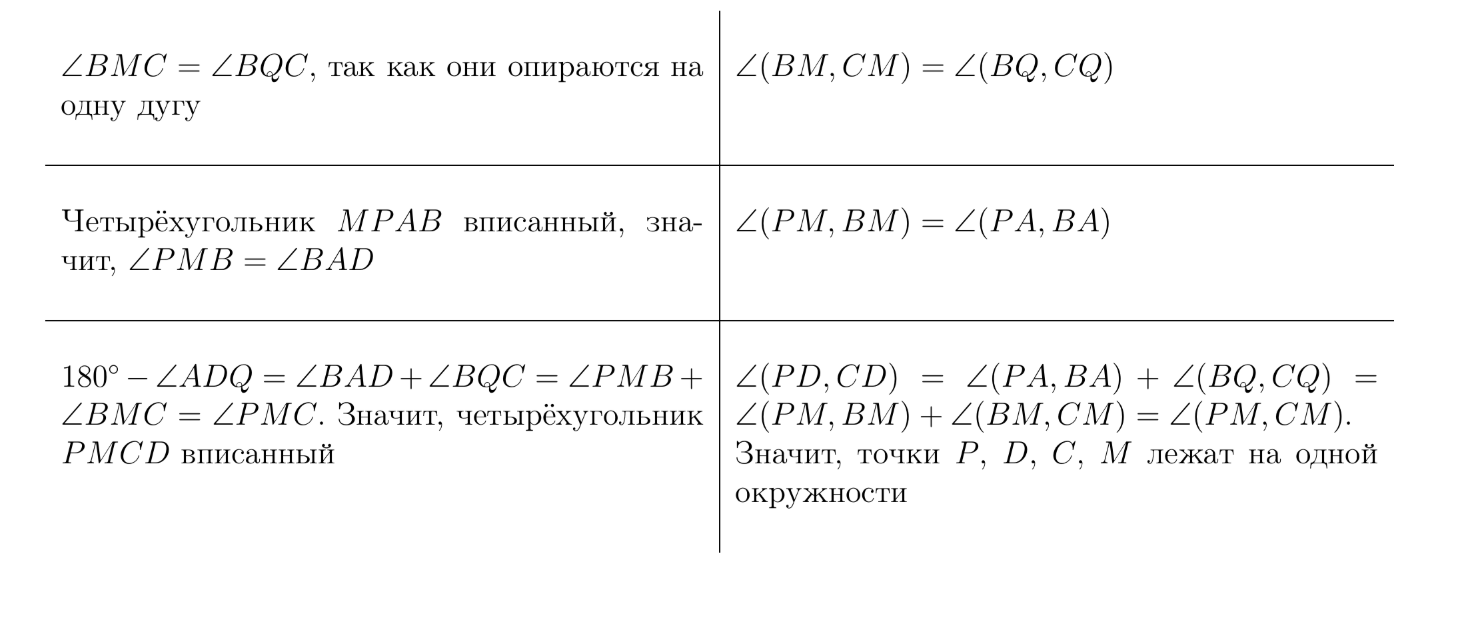
\includegraphics[width=1.05\textwidth]{ЭлМШ 2025-2026/I блок/10/VII/mpt_4.png}
\end{center}

\newpage

\hspace{3mm}

\textbf{\Large Точка Микеля и прямая Обера}

Если на плоскости даны четыре прямые общего положения, существует единственная парабола, которая их касается.

\begin{figure}[h]
    \centering
    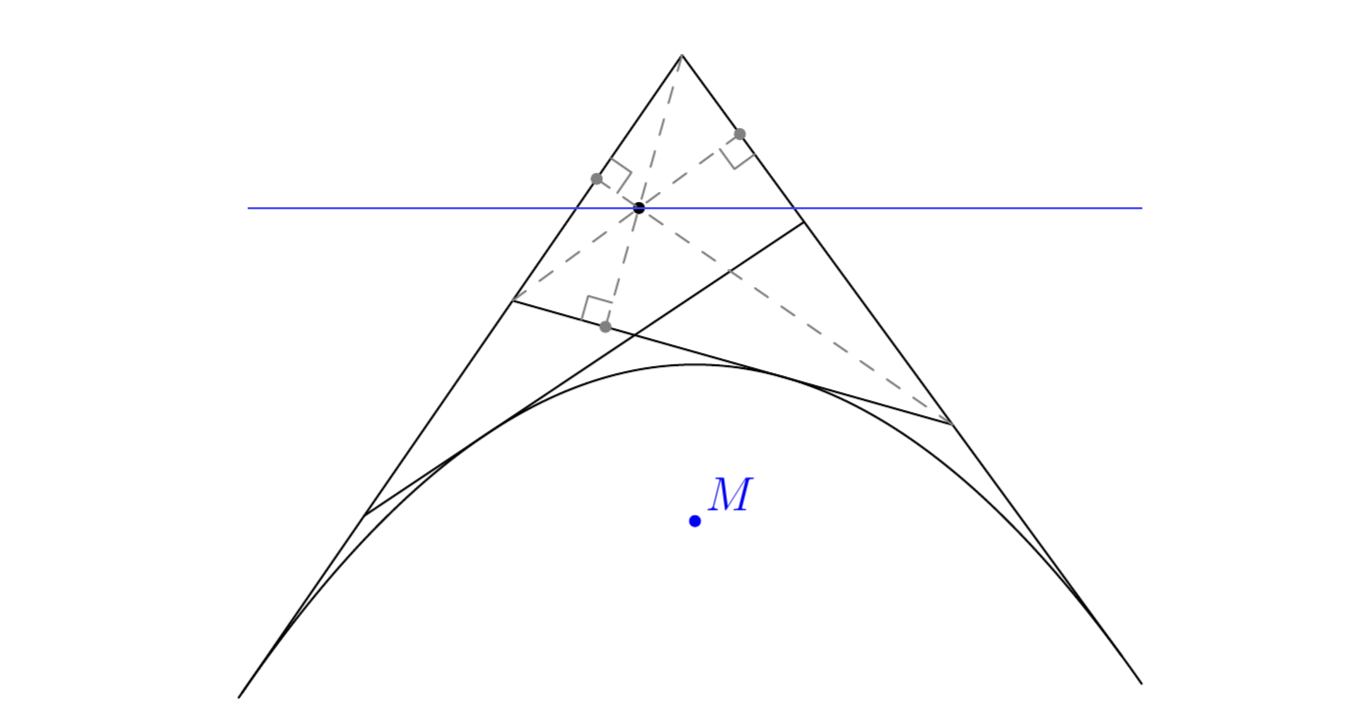
\includegraphics[width=0.8\linewidth]{ЭлМШ 2025-2026/I блок/10/VII/mpt_5.png}
    \caption{}
    \label{fig:placeholder}
\end{figure}

Это следует из того, что пять прямых общего положения однозначно задают невырожденную конику, которая их касается, и того факта, что парабола --- единственная коника, касающаяся бесконечно удалённой прямой.

Фокус этой параболы --- это точка Микеля. Директриса рассматриваемой параболы --- прямая Обера, то есть прямая, проходящая через ортоцентры высекаемых прямыми треугольников. Это следует из того, что ортоцентр описанного около параболы треугольника лежит на её директрисе.